\chapter{Hardware Model and Implementation}

This chapter details the hardware designed during this Master's thesis to accelerate neural network training. The current hardware implements both training and inference acceleration for the neural network architecture described in section \ref{net-arch}.
\todo[inline]{Refer to github, appendix, and project link}
\section{Specifications}
The hardware model was implemented using a ZedBoard. The ZedBoard is a development board equipped with a Zynq-7000 XC7Z020 SoC. The Zynq series has both a processing system and programmable logic, where the processing system is a ARM Cortex-A9 based processor (hereafter referred to as the ``PS'') and the programmable logic is an Artix-7 series FPGA. Bitstreams for the FPGA were generated using Vivado 2018.3 and PetaLinux boot images for the PS were created using Xilinx SDK. The hardware description language (HDL) code for the project was primarily written in SystemVerilog. The programs run on the PS were written in C.

\section{The Implemented Neural Network}\label{net-arch}
The classical MNIST handwritten digit dataset was chosen as the problem setting for the hardware model as a proof-of-concept. This problem has been chosen to verify the value in designing accelerators that take advantage of the finer-grained parallelism present in neural networks. The network consists of an input layer, 3 fully-connected layers, and a softmax output layer. The input layer is a 28$\times$28 grayscale image of a handwritten digit. The dimensions of the rest of the layers in the network are shown in table \ref{net-arch-table}. Layers whose name starts with FC are fully-connected layers.
 
\begin{table}
	\centering
	\begin{tabular}{|c| c| c|}
		\hline
		\textbf{Layer Name}	& \textbf{Input Size} & \textbf{Output Size}\\\hline
		FC0	& 784 (28$\times$28) & 98 \\\hline
		FC1 & 98 & 64 \\\hline
		FC2 & 64 & 10 \\\hline
		Softmax & 10 & 10\\\hline
	\end{tabular}
	\caption{The hidden and output layers in the implemented neural network}
	\label{net-arch-table}
\end{table}

Note that in this implementation, while biases are supported for forward computation, they are not used as the MNIST dataset is already fairly normalized. As such, the biases read are always 0 during the forward pass, and during the backward pass, no updates or gradients are calculated for the bias. Note that the gradient of the bias would just be the gradient of the neuron, unless the neuron had a ReLU activation function with negative net, so implementing this update would be trivial as all neuron gradients are already calculated. 


\section{Design Goals}
There were a few key principles that guided the overall design process throughout the development of the hardware accelerator. A core tenet was to maintain the project such that in the future HDL could be generated for training a network of any architecture so long as the desired layer types had an implementation. As a result, all layers have been modularized and internal components are parameterized. Designing in a modular and parameterizable fashion also allows for quick and easy readjustments to the neural network architecture if needed.
\par 
In addition, optimal usage of resources available was prioritized. For example, the limiting FPGA resource was the amount of digital signal processing slices (DSPs). Therefore, the FPGA design optimized the distribution of DSPs over other resources as opposed to saving an extra Block RAM (BRAM) block. 

\section{Overall Architecture}
In the hardware model, both the Zynq's PS and the FPGA were used to facilitate a cohesive and efficient architecture to accelerate neural network computation. The overall system architecture can be seen in figure \ref{overall-arch}. 

Through memory-mapped I/O, the PS transfers neural net hyperparameters, training data, and control signals to the FPGA. The FPGA transfers training statistics and state data back to the PS. The interface is further described in sections \ref{az-com} and \ref{mmio-lay}.

Inside the FPGA, the neural network described in section \ref{net-arch} is implemented. Layers are connected in both forward and backward directions in order to support training. There are three types of primary modules in the top-level of the FPGA: fully-connected layers, interlayer activation buffers, and the softmax layer. In addition, there is a general control flow in the top-level with which all the primary modules interact.

\begin{figure}
	\centering 
	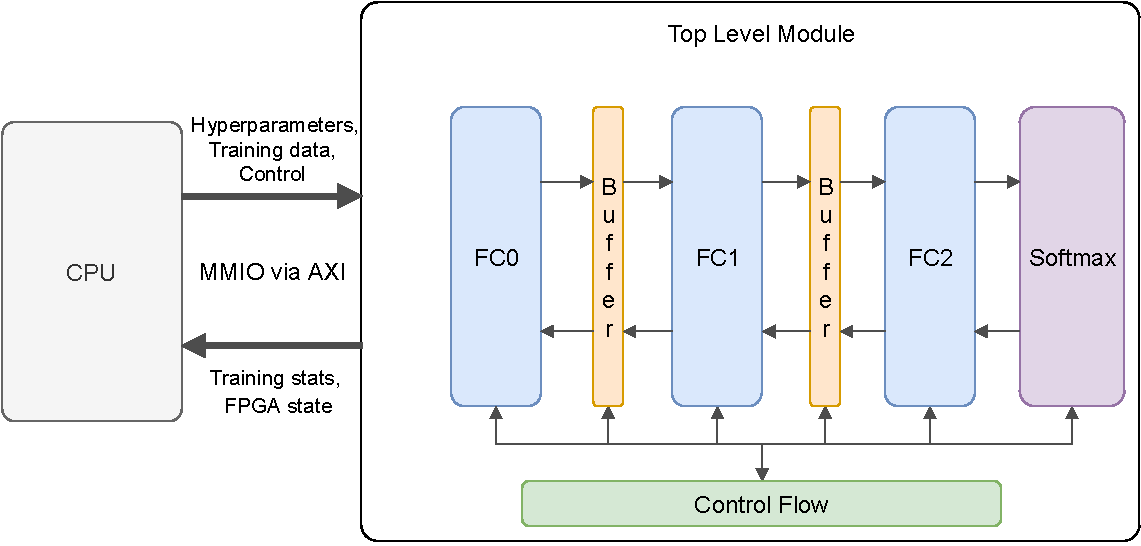
\includegraphics[width=\textwidth]{figures/overall_arch}
	\caption{Architecture of the hardware accelerator}\label{overall-arch}
\end{figure}

\section{Computational Precision}
In this implementation, a bit-width of 18 was chosen for all weight gradients and activations. This value was chosen because the multiplication portion of DSP slices have an input multiplicands with bit widths of 25 and 18 \todo[inline]{cite dsp}. This thesis uses the Q number format to define precision types. For example, Q10.6 would mean that a 16-bit value has 10 integer bits and 6 fractional bits \cite{q-format}. For this accelerator, activations have a precision of Q6.12. Weights and weight gradients both have a precision of Q1.17. These values were chosen through experimental analysis of minimum and maximum activation, weight, and gradients values using the software model described in chapter \ref{ch-sw-model}.

\section{Module Architecture}
As mentioned in the design goal section, one of the tenets of this design was to allow for modularity and parameterization, such that changing a network architecture would not require too much work. As such, there are a few global parameters defined, such as the amount of bits specified for the fixed-point precision. There are also parameters defined for each of the fully-connected layers. These parameters can all be found in the \textit{sys\_defs.vh} file in the Appendix \todo[inline]{fpga appendix}, or on GitHub. 



\subsection{Fully-Connected Layers}
The fully-connected layer modules implement both forward and backward passes. The general architecture is shown in figure \ref{fc-arch}. As DSP slices are limited, both the forward and backward computational units make use of the same resources to compute multiplications, known as the kernel pool. There are 4 modes of computation in the fully-connected layer: forward pass, backpropagating neuron gradients, computing weight gradients, and updating the weights. Of these 4 modes of computation, all except updating the weights make use of the kernel pool. This is because updating the weights makes uses of bit shifting instead of multiplication to multiply gradients by the learning rate.
\begin{figure}
	\centering 
	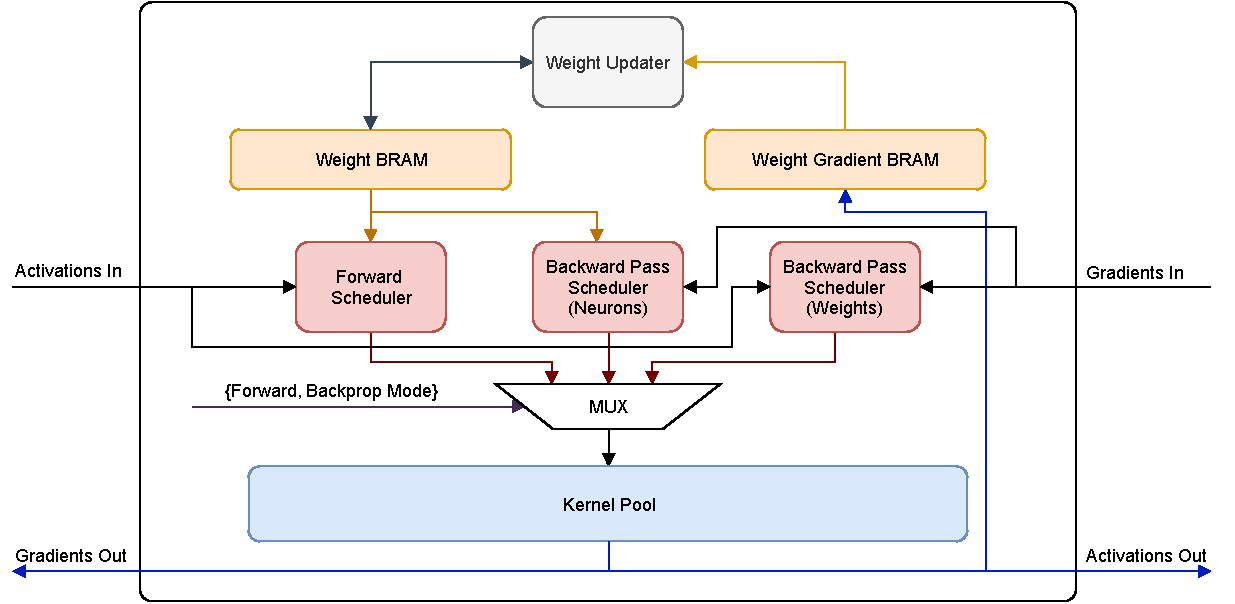
\includegraphics[width=\textwidth]{figures/fully_connected_arch}
	\caption{Architecture of the fully connected layer}\label{fc-arch}
\end{figure}

The forward pass multiplies weights and input activations to produce output activations. Backpropagating neuron gradients multiplies weights by current layer input gradients to produce previous layer gradients as output. The weight gradient computation mutliplies input activation from the forward pass by the current layer gradient, and then writing the computed gradient to the weight gradient BRAM. 

Since being flexible and modular was one of the design goals, all the fully-connected layers use the same kernel and scheduler modules, with different parameters in the instantiation.

\paragraph{Scheduling}
Each of the computational modes needs to have a scheduler to generate addresses to be read and guide the computation. For this, the a generalized scheduler module was implemented. The scheduler uses two pointers starting from the head and middle of the BRAM, and iterates through the entirety during the forward pass. Since the weight BRAMs of each layer are different, certain parameters are assigned for instantiations of the scheduler are also different.

\begin{lstlisting}[
caption={The instantiation of the scheduler for the FC1 layer}, label={sch_instant}, language=SystemVerilog, upquote=true]
fc_scheduler #(.ADDR(`FC1_ADDR), 
	.BIAS_ADDR(`FC1_BIAS_ADDR),
	.MID_PTR_OFFSET(`FC1_MID_PTR_OFFSET), 
	.FAN_IN(`FC1_FAN_IN)) 
	fc1_scheduler_i (
	//inputs
	.clk(clk),
	.rst(rst),
	.forward(forward),
	.valid_i(sch_valid_i),	
	//outputs
	.head_ptr(head_ptr),
	.mid_ptr(mid_ptr),
	.bias_ptr(bias_ptr),
	.has_bias(sch_has_bias)
);		
\end{lstlisting}
The instantiation of the scheduler shown in listing \ref{sch_instant} is similar across all the 3 fully connected layers, with only the parameters in the instantiations differing. The outputs are the pointers whose starting addresses are at the head and middle of the weight BRAM. In addition, there is a bias pointer and a signal to indicate if there is a bias.


\paragraph{Kernel}
The same kernel module is used in all the fully-connected layers. A high-level architecture of the computational kernel is provided in figure \ref{kernel-arch}. Note that saturation checking is not shown in the figure for simplicity, though it is implemented and verified. The scarcest computational resource in this FPGA architecture are the DSP slices, thus the kernel has been designed so that all required forms of multiplication are supported in the network. This is why there are 3 different outputs.

\begin{figure}
	\centering 
	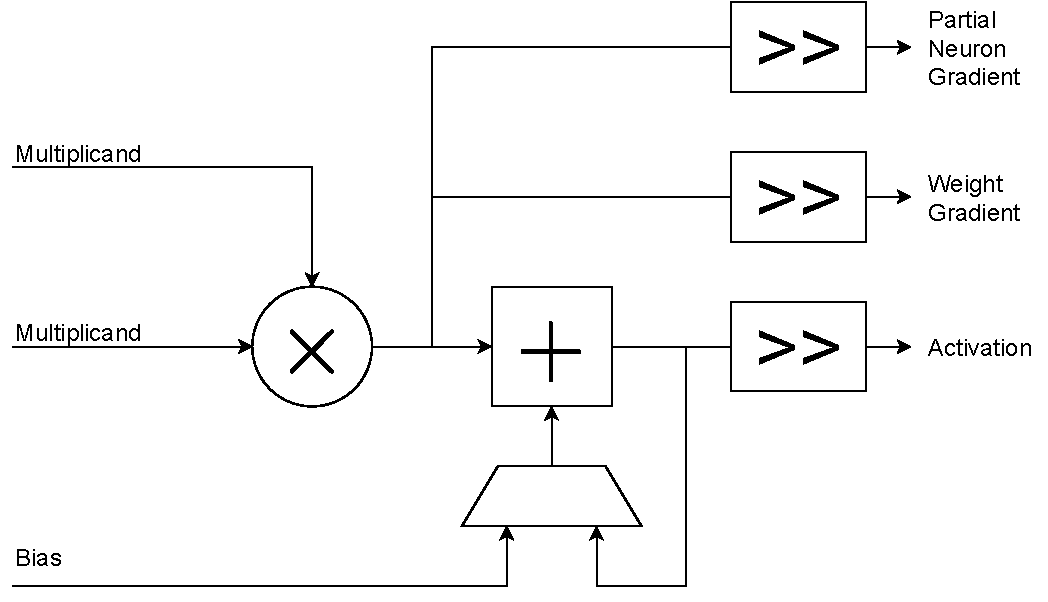
\includegraphics[width=5in]{figures/kernel_arch}
	\caption{Architecture of the kernel, saturation checking not shown.}\label{kernel-arch}
\end{figure}

From the figure, the top output is the neuron gradient. This multiplies a weight with a gradient. Multiplying two Q1.17 values results in a Q2.34 product, which must be checked for saturation in the top 2 bits and the bottom 17 bits must be truncated to obtain a Q1.17 output.

The middle output is the weight gradient. The weight gradients computation multiplies a gradient with an activation. As gradients are Q1.17 and activations are Q6.12, the output is Q7.29. To convert the resultant Q7.29 result to the desired Q1.17 format required for a weight gradient, the top 7 bits must be checked for saturation and the bottom 12 bits truncated. 

Finally, the bottom output is the net output calculated during the forward pass. This value becomes valid after performing $n$ MACs, where $n$ is the fan-in of a neuron. An input activation and corresponding weight are multiplied and added to either a bias or the running sum for the current in-progress net calculation. 

Since the forward pass multiplies Q6.12 activations by Q1.17, the multiplied result is 36-bits, Q7.29. Since for some layers fan-in can be quite large, extra precision is used during the accumulation phase. The accumulated sum uses 32 bits: Q6.26, thus the internal sum must be checked for saturation and truncation of the bottom 3 bits for each MAC. The conversion from the internal sum precision of Q6.26 to the net output of Q6.12 is a simple truncation of the bottom 14 bits.

With this amount of internal precision during the forward pass, truncation during the internal summation has much less effect on the precision than the final truncation to 18 bits for when the neuron net is computed. The largest fan-in in this network is 784 in the FC0 layer. For each internal MAC, the 27th fractional bit onward is truncated when converted from the product with precision Q7.29 to the internal sum precision of Q6.26. Assuming that the 27th bit equally probable to be 0 or 1, then the 27th bit is 1 approximately half of the time. This means that the average truncation per MAC is $0.5 \times 2^{-27} = 2^{-28}$. Given the 784 MACs of layer FC0, the expected truncation error is $784 \times 2^{-28} = 2.92\times{10^{-6}}$. The final truncation error from Q6.26 to Q6.12 truncates from the 13th fractional bit, resulting in an expected truncation error of $2^{-14} = 6.1\times10^{-5}$. Thus, truncation error from internal summation is expected to be more than 20 times less than the truncation to the 18-bit net output. Therefore, truncation error is successfully minimized during the internal summation of net computation during the forward pass.
\todo[inline]{should this go in the analysis section? yeah probably}



\paragraph{BRAM Layout}

\paragraph{Weight Updates}

\subsubsection{Individual Fully-Connected Layer Implementation}
While the modules used for the 


\subsection{Interlayer Architecture}
\begin{figure}
	\centering 
	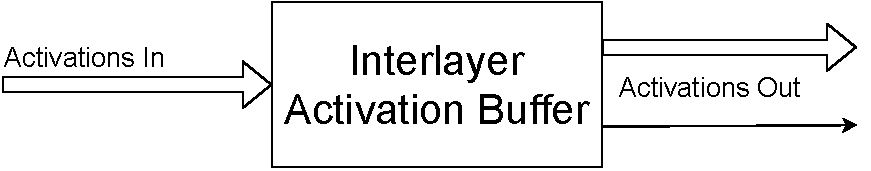
\includegraphics[width=\textwidth]{figures/interlayer_buffer}
	\caption{The interlayer buffer}\label{softmax-arch}
\end{figure}

\subsection{Softmax Layer}
\begin{figure}
	\centering 
	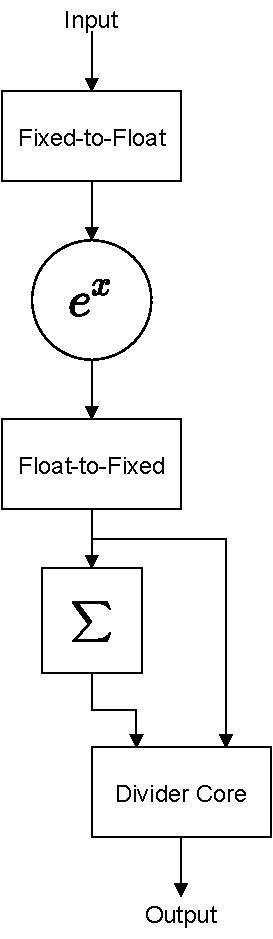
\includegraphics{figures/softmax}
	\caption{Architecture of the softmax layer}\label{softmax-arch}
\end{figure}

To have training be feasible, a proper loss function was required to calculate initial gradients for the output neurons. As such, cross entropy loss, one of the most popular loss functions in deep learning was chosen for this network. Cross-entropy loss is a statistical loss that uses probabilities as input, as shown below.



\begin{align}
\mathcal{L}(y) = - \sum_{i = 1}^{C}y_{i,c}\log(p_{i,c})
\end{align}
In this equation, 
\todo[inline]{Consider against the cross entropy loss defined in chapter 3, define it in chapter 2 IMO}

As explained in chapter \ref{background}, the softmax functions converts logits to probabilities in following manner

\section{PS-FPGA Communication}\label{az-com}
ps master fpga slave

\subsection{Memory Map Layout}\label{mmio-lay}
The memory map may be extended easily by adding or modifying address definitions to the AXI slave connected to the PS in the FPGA. In the PS code, one only need modify the \texttt{ddr\_data} struct definition found in the C files of the PS source code. The memory map layout is defined in table \ref{tbl:mmio}. All addresses have a base address of 0x40000000. Note that values with addresses starting from 0x0 to 0x18 are registers written to by the FPGA. Values with addresses starting from 0x1C until 0x343 are written to by the PS. Output data from the FPGA is provided in the address range of 0x344 -- 0x358.
\begin{table}
	\centering
	\Large PS -- FPGA Memory Map \\\vspace{0.5em}
	\normalsize
	\begin{tabularx}{\textwidth}{|l| l| X|}
		\hline
		\textbf{Offset}	& \textbf{Name} & \textbf{Brief Description}\\\hline
		
		\texttt{0x0}	& 
		\texttt{fpga\_img\_id} & 
		The ID of the image that the FPGA is currently processing. \\\hline
		
		\texttt{0x4} &
		\texttt{epoch} &
		The current epoch in the FPGA \\\hline
		
		\texttt{0x8} &
		\texttt{num\_correct\_train} &
		The amount of correctly classified training images during the current epoch. \\\hline 
		
		\texttt{0xC} &
		\texttt{num\_correct\_test} &
		The amount of correct classified test images during the current epoch. \\\hline
		
		\texttt{0x10} &
		\texttt{idle\_cycles} &
		The amount of idle cycles in the FPGA since the start signal was received from the PS. An idle cycle is one in which none of the layers are performing any form of computation. \\\hline
		
		\texttt{0x14} &
		\texttt{active\_cycles} &
		The amount of active cycles in the FPGA since the start signal was received from the PS. An active cycle is one in which at least one of the layers is performing computations. \\\hline
		
		\texttt{0x18} &
		\texttt{status} &
		A 32-bit register with many different flags from the FPGA, such as the layer states, for example. \\\hline 
		
		\texttt{0x1C} &
		\texttt{start} &
		The start signal for training. \\\hline 
		
		\texttt{0x20} &
		\texttt{n\_epochs} &
		The number of epochs to train for in the FPGA \\\hline 
		
		\texttt{0x24} &
		\texttt{learning\_rate} &
		Value set to specify the amount of right shifts weight gradient should incur before updating a weight. \\\hline 
		
		\texttt{0x28} &
		\texttt{training\_mode} &
		Specifies whether the backward pass should be performed or not during computation.\\\hline
		
		\texttt{0x2C} &
		\texttt{img\_set\_size} &
		The size of the image set used during computation. \\\hline 
		
		\texttt{0x30} &
		\texttt{img\_label} &
		The label of the current image being computed. \\\hline 
		
		\texttt{0x34 -- 0x343} &
		\texttt{img} &
		Image data for the FPGA. \\\hline
		
		\texttt{0x344 -- 0x358} &
		\texttt{output} &
		Output data from the last layer in the FPGA, before the softmax function is performed, so they are still logits in this case.\\\hline		
	\end{tabularx}	
	\caption{Current memory map for communication between the PS and the FPGA.}
	\label{tbl:mmio}
\end{table}


\section{Training Cycle Dataflow}

\section{Project Structure}


\begin{figure}
	\begin{tikzpicture}[]
	\node[] at (0,0) (top) {neural\_net\_top.sv};
	\node[] at (3, -1) (mlled) {fc0\_layer.sv};
	\node[] at (3, -2) (debounce) {debounce.v};
	\node[] at (3, -3) (scope) {red\_pitaya\_scope.v};
	\node[] at (3, -4) (buffermodule) {buffer\_module.v};
	\node[] at (3, -5) (irf) {internal\_ref\_gen.xci};
	\node[] at (3, -6) (pfd) {pfd.v};
	\node[] at (6, -7) (pfdblock) {pfd\_block.v};
	\node[] at (6, -8) (pfdfilter) {pfd\_filter.v};
	\node[] at (3, -9) (freqcounter) {freq\_counter.v};
	\node[] at (6, -10) (freqcounterblock) {freq\_counter\_block.v};
	\node[] at (9, -11) (interp) {freq\_interp\_clk.xci};
	\node[] at (3, -12) (pid) {red\_pitaya\_pid.v};
	\node[] at (6, -13) (pidblock) {imra\_pid\_block.v};
	\node[] at (6, -14) (pidfilt) {iir\_filter.v};
	\node[] at (3, -15) (analog) {red\_pitaya\_analog.v};
	\node[] at (6, -16) (dds) {dds/mixer/lpf};
	
	
	\draw [->] (top) |- (mlled.west);
	\draw [->] (top) |- (debounce.west);
	\draw [->] (top) |- (scope.west);
	\draw [->] (top) |- (buffermodule.west);
	\draw [->] (top) |- (irf.west);
	\draw [->] (top) |- (pfd.west);
	\draw [->] (top) |- (freqcounter.west);
	\draw [->] (top) |- (pid.west);
	\draw [->] (top) |- (analog.west);
	\draw [->] (pfd) |- (pfdblock.west);
	\draw [->] (pfd) |- (pfdfilter.west);
	\draw [->] (freqcounter) |- (freqcounterblock.west);							
	\draw [->] (freqcounterblock) |- (interp.west);
	\draw [->] (pid) |- (pidblock.west);
	\draw [->] (pid) |- (pidfilt.west);
	\draw [->] (analog) |- (dds.west);
	
	
	
	\end{tikzpicture}
	\caption{Hierarchy of the FPGA code used for the implementation of the network.}
\end{figure}